\chapterauthor{Jeferson J. Lima}{Departamento de Informática (DAINF) \\Universidade Tecnológica Federal do Paraná (UTFPR)}
\chapter{Conceitos Básicos}

 
\section{Introdução}\label{intro::cap3}

As técnicas de localização aplicadas na robótica móvel fornecem uma estimativa da posição do um robô em relação as coordenas iniciais, sendo este um mapa ou qualquer outro modelo de referência.

A percepção destas coordenadas se dá através de uma série de sensores que fornecem um estimativa da localização o robô durante determinado movimento. Esse predição do estado é executada interativamente em intervalos de tempo, determinados pela frequência de operação dos sensores. 

Assim, a crença do estado atual pode ser encontrada e os dados adqueridos dos sensores, podem então, ser traduzidos em mapas a qual o mesmo robô ou outros robôs podem recorrer para melhorar a crença da posição atual.

\section{Filtro de Bayes}

O Filtro de Bayes é o algoritmo em diversas técnicas de auto-localização onde pretende-se resolver a manutenção da crença da posição de um robô, com base nos seus estados. O algoritmo calcula a densidade de probabilidade que se traduz na crença do robô a partir de dados dos sensores e o modelo de controle do robô  \cite{thrun2006probalistic}. A solução deste problema de auto-localização, utilizando-se da inferência bayesiana, está em encontrar o valor esperado da posição em cada instante de tempo, conforme a equação Eq. \ref{eq:bayes1}.

\begin{equation}
    \label{eq:bayes1}
    \hat X_t = E\left[X_t| z_t, u_t\right] = \displaystyle \int\limits_x x P(X_t = x| z_t, u_t)\text{d}x
\end{equation}


Para este problema, o algoritmo do Filtro de Bayes apresenta-se como uma forma recursiva, Eq. \ref{eq:bayes2}, onde $\text{Bel}(x_t)$ representa a função densidade da crença no tempo $t$ e $\text{Bel}(x_{t-1})$ a função no intervalo de tempo anterior. A relação entre o intervalo de tempo das interações do filtro, será definida, conforme citado acima pela velocidade de operação dos sensores envolvidos, aqui apresentados como $z_t$. O termo $u_t$ representa a variável de ação do modelo ou variável de controle.


\begin{equation}
    \label{eq:bayes2}
    \text{\text{Bel}}(x_t) = \eta P(z_t| x_t) \int P(x_t| u_t, x_{t-1}) \text{Bel}(x_{t-1})\text{d}x_{t-1}
\end{equation}


A esta primeira fase do algoritmo, a qual calcula a distribuição em relação a crença dos estados $x_{t-1}$ e $u_t$, é chamada de predição e o resultado da função crença é dada por $\overline{\text{Bel}}(x_t)$.

Na segunda fase, chamada aqui de correção, a crença $\overline{\text{Bel}}(x_t)$ é multiplicada pela probabilidade dos estados observados em relação ao sensores $z_t$.

\begin{algorithm}[H]
    \caption{Filtro de Bayes}
    \begin{algorithmic}[1]
    \Procedure{predição}{$\text{Bel}(x_{t-1}), u_t$}
        \State $\overline{\text{Bel}}= \displaystyle\int P(x_t| u_t, x_{t-1})\text{Bel}(x_{t-1})\text{d}x_t$
    \EndProcedure
    \Procedure{Correção}{$\overline{\text{Bel}}(x_{t}), z_t$}
        \State ${\text{Bel}}= \displaystyle\textcolor{white}{\int}  \eta P(z_t| x_{t})\overline{\text{Bel}}(x_{t})$
    \EndProcedure
    \State Normatiza $\eta \displaystyle\int \text{Bel}(x_t)\text{d}x_t = 1$
    \State \textbf{Retorne} $\text{Bel}(x_t)$

    \end{algorithmic}
\end{algorithm}

O algoritmo finaliza com a crença normatizada e a estimativa da posição do robô é calculada. O algoritmo do Filtro de Bayes apresentado aqui é aplicável apenas a uma classe de problemas simples, no entanto serve de base para implementações mais complexas onde a cinemática e dinâmica do sistemas são consideradas, como no exemplo do Filtro de Kalman a ser apresentado abaixo.

\section{Filtro de Kalman}

O Filtro de Kalman é provavelmente a implementação mais aplicada com base no Filtro de Bayes. Proposto por Rudolph Emil Kalman, em 1950 como técnica para filtragem e predição de sistemas lineares. O Filtro proposto por Kalman resolve o problema de observação dos sensores externos do robô, considerando inerentes a leitura dos sensores. \cite{thrun2006probalistic,romero2014robotica}.

A garantia da densidade de probabilidade, apresentada em Eq. \ref{eq:bayes2}, é dada por uma aproximação do método apresentado anteriormente. Nesta aproximação o modelo de movimento do robô e o modelo do observador, com base nos sensores, é representado por densidades gaussianas multivariáveis.

A função de densidade gaussiana $P(X = x)$, sendo um $X$ um vetor, pode ser expressa na seguinte forma ${P(X = x) \sim N(\mu, \sigma^2)}$, onde $\mu$ representa a média e $\sigma^2$ a variância da distribuição, conforme a equação Eq. \ref{eq:gauss1}.

\begin{equation}
    \label{eq:gauss1}
    P(X = x) = \dfrac{1}{\sqrt{2\pi\sigma^2}}\cdot 
    \exp\left\{-\frac{(x-\mu)^2}{2\sigma^2}\right\}
\end{equation}

A Figura \ref{fig::gauss1} apresenta três funções de densidade gaussiana, com os valores respectivamente para $\mu_i = \{0,0,-2\}$ e $\sigma^2_i = \{1,2,1\}$.


\begin{figure}[!ht]
    \centering
    \begin{tikzpicture}[
    declare function={
      normalpdf(\x,\mu,\sigma)=
      (2*3.1415*\sigma^2)^(-0.5)*exp(-(\x-\mu)^2/(2*\sigma^2));
    },
    hplot/.style={ycomb, mark=o, dashed}, ,scale=0.8]
  
    \begin{axis}[
      width=12cm, height=6cm,
      samples=50,
      xlabel=$x$, ylabel=$p(x)$,
      xlabel style={at={(1,0)}, anchor=north west},
      ylabel style={rotate=-90, at={(0,1)}, anchor=south east},
      legend style={draw=none, fill=none},
      domain=-6:9,
      legend cell align=left,
      xmin=-7, xmax=11]
  
      \addplot [smooth, thick] {normalpdf(x,0,1)}
      node[pos=0.47, pin={right:$\mu=0,\sigma^2=1$}] {};
      \addplot [smooth, blue] {normalpdf(x,0,2)}
      node[pos=0.6, pin={45:$\mu=0,\sigma^2=2$}] {};
      \addplot [smooth, red] {normalpdf(x,-2,1)}
      node[pos=0.25, pin={[text centered, text width=8ex]
        200:$\mu=-1$, $\sigma^2=1$}] {};
  
      \addplot [hplot, samples at={0}] {normalpdf(x,0,1)};
      \addplot [hplot, samples at={0}, blue] {normalpdf(x,0,2)};
      \addplot [hplot, samples at={-2}, red] {normalpdf(x,-2,1)};
  
      \node[anchor=north east] at (axis description cs: 0.975,  0.95)
      {$p(x) = \dfrac{1}{\sqrt{2\pi\sigma^2}}\cdot 
        \exp\left\{-\frac{(x-\mu)^2}{2\sigma^2}\right\}$};
  
    \end{axis}
  \end{tikzpicture}
    \caption{Representação de três funções de Distribuição Normal}
    \label{fig::gauss1}
\end{figure}

Um dos requisitos para aplicação do Filtro de Kalman é que o modelo determinístico de observação se haja linear para que haja uma correta aproximação com a densidade de probabilidade, conforme é mostrado na equação Eq. \ref{eq::linear1d}.


\begin{equation}
    \label{eq::linear1d}
    \left.
    \begin{aligned}
            X & \sim N\left(\mu, \sigma^2\right)\\
            Y & = aX + b\\
    \end{aligned} \right\}
    \quad \Rightarrow \quad Y \sim N\left(a\mu+b\right)
\end{equation}

Os coeficientes $a$ e $b$ são coeficientes lineares do modelo. A equação Eq. \ref{eq::linear1d} possui apenas um estado, no entanto sistemas complexos são tipicamente representados diversos estados e diversos sensores.
Sistemas robóticos possuem vários estados, sendo assim a densidade de probabilidade ${P(\mathbf{x}) \sim N(\boldsymbol{\mu}, \textstyle\sum)}$ é formada por uma equação multivariável, onde $\boldsymbol{\mu}$ representa o vetor das médias e ${\textstyle\sum}$ a matriz de covariância, conforme pode ser visto na Equação \ref{eq::linearNd}.

\begin{equation}
    \label{eq::linearNd}
    P(\mathbf{x}) = \frac{1}{\sqrt{(2\pi)^d\|\textstyle\sum\|}}\exp\left\{-\frac{1}{2} (\mathbf{x}-\boldsymbol\mu)^T\textstyle\sum{}^{-1}(\mathbf{x}-\boldsymbol\mu)\right\}
\end{equation}

Desta forma, a Figura \ref{fig::gauss2} apresenta a distribuição normal para um sistema bivariável.


\begin{figure}[!ht]
    \centering
    \resizebox{0.6\textwidth}{!}{
\pgfplotsset{%
  colormap={whitered}{color(0cm)=(white);
  color(1cm)=(orange!75!red)}
}
\begin{tikzpicture}[
  declare function = {mu1=1;},
  declare function = {mu2=2;},
  declare function = {sigma1=0.5;},
  declare function = {sigma2=1;},
  declare function = {normal(\m,\s)=1/(2*\s*sqrt(pi))*exp(-(x-\m)^2/(2*\s^2));},
  declare function = {bivar(\ma,\sa,\mb,\sb)=
    1/(2*pi*\sa*\sb) * exp(-((x-\ma)^2/\sa^2 + (y-\mb)^2/\sb^2))/2;},scale=0.6]
  \begin{axis}[
    colormap name  = whitered,
    width          = 15cm,
    view           = {45}{65},
    enlargelimits  = false,
    grid           = major,
    domain         = -1:4,
    y domain       = -1:4,
    samples        = 26,
    xlabel         = $x_1$,
    ylabel         = $x_2$,
    zlabel         = {$P$},
    colorbar,
    colorbar style = {
      at     = {(1,0)},
      anchor = south west,
      height = 0.25*\pgfkeysvalueof{/pgfplots/parent axis height},
      title  = {$P(x_1,x_2)$}
    }
  ]
    \addplot3 [surf] {bivar(mu1,sigma1,mu2,sigma2)};
    \addplot3 [domain=-1:4,samples=31, samples y=0, thick, smooth]
      (x,4,{normal(mu1,sigma1)});
    \addplot3 [domain=-1:4,samples=31, samples y=0, thick, smooth]
      (-1,x,{normal(mu2,sigma2)});

    \draw [black!50] (axis cs:-1,0,0) -- (axis cs:4,0,0);
    \draw [black!50] (axis cs:0,-1,0) -- (axis cs:0,4,0);

    \node at (axis cs:-1,1,0.18) [pin=165:$P(x_1)$] {};
    \node at (axis cs:1.5,4,0.32) [pin=-15:$P(x_2)$] {};
  \end{axis}
\end{tikzpicture}}
    \caption{Distribuição Normal Bivariável}
    \label{fig::gauss2}
\end{figure}

Desta forma, a densidade de probabilidade, conforme é mostrado na equação abaixo:

\begin{equation}
    \left.
    \begin{aligned}
            X & \sim N\left(\boldsymbol\mu, \textstyle\sum\right)\\
            Y & = AX + B\\
    \end{aligned} \right\}
    \quad \Rightarrow \quad Y \sim N\left( A\boldsymbol\mu+B, A\textstyle\sum A^T \right)
\end{equation}

Para o caso multivariável, $A$ e $B$ são matrizes $n \times n$ e $n \times l$, respectivamente, sendo $n$ o número de estados e $l$ o número de variáveis de controle.


\begin{itemize}
    \item Num \textcolor{blue}{modelo determinístico} o resultado do sistema é pré determinado em função dos dados de entrada, exemplo:
    \begin{align*} 
        x_t &= A_t x_{t-1} + B_t u_t\\ 
        z_t &= C_t x_t
    \end{align*}
    \item Num \textcolor{blue}{modelo estocástico} o resultado do sistema não depende somente dos dados de entrada, mas também de outros fatores, normalmente
    aleatórios:
    \begin{align} 
        x_t &= A_t x_{t-1} + B u_t +  w_t\\ 
        z_t &= C_t x_t + v_t
    \end{align}
    \begin{itemize}
        \item $A_t$ Matriz $(n \times n)$ que descreve os estados do modelo.
        \item $B_t$ Matriz $(n \times l)$ que descreve os estados do controle.
        \item $C_t$ Matrix $(k\times n)$ sendo os estados de $x_t$.
        \item $ w_t$ Variável aleatória do processo com distribuição normal e covariância $Q_t$.
        \item $v_t$ Rúido aleatório com distribuição normal e covariância de $R_t$.
    \end{itemize}
\end{itemize}


Representação Grafica
    
    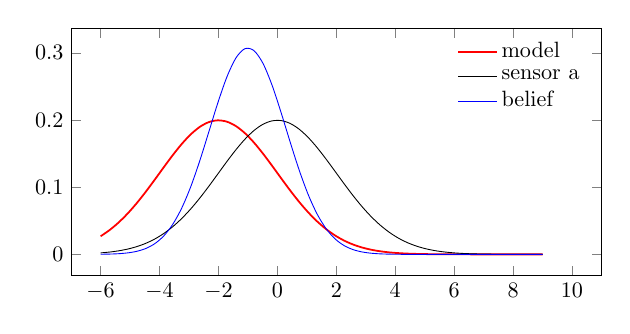
\begin{tikzpicture}[
      declare function={
        normalpdf(\x,\mu,\sigma)=
        (2*3.1415*\sigma^2)^(-0.5)*exp(-(\x-\mu)^2/(2*\sigma^2));
      },
      hplot/.style={ycomb, mark=o, dashed}, ,scale=0.8]
    
      \begin{axis}[
        width=10cm, height=5.5cm,
        samples=50,
        legend style={draw=none, fill=none},
        domain=-6:9,
        legend cell align=left,
        xmin=-7, xmax=11]
    
        \addplot [smooth, thick, red] {normalpdf(x,-2,2)} node[] {};
        \addplot [smooth, black]      {normalpdf(x,0,2)} node[] {};
        \addplot [smooth, blue]       {normalpdf(x,-1,1.3)} node[] {};
        \legend{model, sensor a, belief};
      \end{axis}
    \end{tikzpicture}


\begin{tabular}{r l}
    $\color{blue}{\text{Bel}}(x_t)$ & = $P(x_t| u_1, z_1,  \cdots, z_t)$ \\
    Bayes & = $\eta P(z_t|x_t,  u_1, z_1,  \cdots,  u_t)P(x_t, u_1, z_1, \cdots, u_t)$ \\
    Markov & = $\eta P(z_t|x_t)P(x_t, u_1, z_1, \cdots, u_t)$ \\
    Prob. Total & = $\eta P(z_t|x_t)\displaystyle\int P(x_t| u_1, z_1, \cdots, u_t,x_{t-1})$ \\
                &  \quad \quad \quad $P(x_{t-1}| u_1, z_1, \cdots, u_t)\text{d}x_{t-1}$\\
    Markov & = $\eta P(z_t|x_t)$ $\displaystyle\int P(x_t| u_t,x_{t-1})P(x_{t-1}| u_1, z_1, \cdots, u_t)\text{d}x_{t-1}$ \\
    Markov & = $\eta P(z_t|x_t)$ $\displaystyle\int P(x_t| u_t,x_{t-1})\color{blue}{P(x_{t-1}| u_1, z_1, \cdots, z_{t-1}})\color{gray}{\text{d}x_{t-1}}$ \\
\end{tabular}   

\begin{equation*}
    \color{blue}{\text{Bel}}(x_t)  \color{gray}{=\eta P(z_t|x_t)\displaystyle\int P(x_t| u_t,x_{t-1})}\color{blue}{\color{blue}{\text{Bel}}(x_{t-1})}\color{gray}{)\text{d}x_{t-1}}
\end{equation*}

Algoritmo
\begin{itemize}
    \item Iniciando as Variável:
    \begin{equation}
        \text{Bel}(x_0) = N\left(x_0, \mu_o, {\textstyle\sum} _0\right)
    \end{equation}
    \item Tempo de convergência do filtro.
\end{itemize}



\begin{itemize}
    \item Com base na equação:
    \begin{equation*}
        \color{blue}{\text{Bel}}(x_t)  \color{gray}{=\eta P(z_t|x_t)\displaystyle\int P(x_t| u_t,x_{t-1})}\color{blue}{\color{blue}{\text{Bel}}(x_{t-1})}\color{gray}{)\text{d}x_{t-1}}
    \end{equation*}
    \item E considerando que o sistema abaixo é linear e observável:
    \begin{equation*}
        \begin{split}
            x_t &= A_t x_{t-1} + B_t u_t\\ 
            z_t &= C_t x_t
        \end{split}
    \end{equation*}
    \item Um sistem é observável se o posto da matriz $\mathcal {O}$ é igual a $n$.
    \begin{equation*}
        \mathcal {O}={\begin{bmatrix}C_t\\C_tA_t\\C_tA^{2}_t\\\vdots \\C_tA^{n-1}_t\end{bmatrix}, \quad \text{rank}(\mathcal {O}}) = n
    \end{equation*}
\end{itemize}



Algoritmo - Prediction
\begin{itemize}
    \item Temos a função de probabilidade do sistema, expressa por:
    \begin{equation*}
        p(x_t| u_t, x_{t-1})= N\left(x_t; A_tx_{t-1}+ B_tu_t, Q_t\right)
    \end{equation*}   
    \item ou seja:
    \begin{equation*}
        \overline{\text{Bel}}(x_t)  = \displaystyle\int\underbrace{P(x_t|u_t, x_{t-1})}_{\sim N\left(x_t; A_t x_{t-1}+ B_tu_t, Q_t\right)} \overbrace{\text{Bel}(x_{t-1})}^{\sim N\left(x_{t-1}; \mu_{t-1}, \textstyle\sum {}_{t-1}\right)}\text{d}x_{t-1}
    \end{equation*}
\end{itemize}


\begin{tabular}{p{1.5cm} l l}
    $\overline{\text{Bel}}(x_t)$  & = $\displaystyle\int P(x_t|u_t, x_{t-1})$ & $\text{Bel}(x_{t-1})\text{d}x_{t-1}$ \\
    & \quad\quad\quad\quad\quad $\Downarrow$ & \quad\quad\quad$\Downarrow$ \\
    & $\sim N\left(x_t; A_t x_{t-1}+ B_tu_t, Q_t\right)$ & $\sim N\left(x_{t-1}; \mu_{t-1}, \textstyle\sum {}_{t-1}\right)$ \\
    & \quad\quad\quad\quad\quad $\Downarrow$ & \\
\end{tabular}


    \begin{equation*}
        P(\mathbf{x}) = \frac{1}{(2\pi)^{\frac{d}{2}\|\sum\|^{\frac{1}{2}}}}\exp\left\{-\frac{1}{2} (\mathbf{x}-\mu)^T\textstyle\sum{}^{-1}(\mathbf{x}-\mu)\right\}
    \end{equation*}        


\begin{tabular}{p{1.2cm} l}
    & $\quad\quad\quad\quad\quad \Downarrow$\\
    $\overline{\text{Bel}}(x_t)$  & = $\eta \displaystyle\int \exp\left\{  -\frac{1}{2} \left(x_t - A_t x_{t-1} - B_t\right)^T Q_t \left(x_t - A_t x_{t-1} - B_t\right)  \right\}$ \\
\end{tabular}

\begin{tabular}{p{2.3cm} l}
    & $\exp\left\{ -\displaystyle\frac{1}{2} \left(x_{t-1} - \mu_{t-1}\right)^T \textstyle\sum {}_{t-1} \left(x_{t-1} - \mu_{t-1}\right)  \right\}\text{d}x_{t-1}$
\end{tabular}    



\begin{itemize}
    \item Continuando ...
\end{itemize}

\begin{tabular}{p{1.2cm} l}      
    $\overline{\text{Bel}}(x_t)$  & = $\eta \displaystyle\int \exp\left\{  -\frac{1}{2} \left(x_t - A_t x_{t-1} - B_t\right)^T Q_t \left(x_t - A_t x_{t-1} - B_t\right)  \right\}$ \\
\end{tabular}
    
\begin{tabular}{p{2.3cm} l}
    & $\exp\left\{ -\displaystyle\frac{1}{2} \left(x_{t-1} - \mu_{t-1}\right)^T \textstyle\sum {}_{t-1} \left(x_{t-1} - \mu_{t-1}\right)  \right\}\text{d}x_{t-1}$
\end{tabular}    


\begin{equation}
    \overline{\text{Bel}} = 
    \left\{
    \begin{aligned}
            \overline{\mu}_t & = A_t\mu_{t-1} + B_t u_t\\
            \overline{\textstyle\sum}_t & = A_t {\textstyle\sum}_{t-1} A_t^T+ Q_t\\
    \end{aligned} \right.
\end{equation}


Algoritmo - Measurement Update
\begin{itemize}
    \item Considerando a saída do sistema:
    \begin{equation*}
        z_t = C_t x_t + \delta_t
    \end{equation*}
    \item Apresentadas as equações lineares do observador de estados, temos a função de probalilidade:
    \begin{equation*}
        P(z_t| x_t)= N\left(z_t; C_t x_t, R_t\right)
    \end{equation*}   
    \item ou seja:
    \begin{equation*}
        \text{Bel}(x_t)  = \eta \underbrace{P(z_t|x_t)}_{\sim N\left(z_t; C_t x_t, Q_t^{-1}\right)} \overbrace{\overline{\text{Bel}}(x_t)}^{\sim N\left(x_t; \overline{\mu}_t, \overline{\textstyle\sum}_t\right)}
    \end{equation*}
\end{itemize}


\begin{tabular}{p{1.5cm} l l l}
    $\text{Bel}(x_t)$  & = $\eta$ & $P(z_t| x_t)$ & $\overline{\text{Bel}}(x_t)$ \\
    & & $\quad \Downarrow$ & $\quad\Downarrow$ \\
    & & $\sim N\left(z_t; C_t x_t, Q_t\right)$ & $\sim N\left(x_t; \overline{\mu}_t, \overline{\textstyle\sum}_t\right)$ \\
    & & $\quad \Downarrow$ &  \\
\end{tabular}

\begin{tabular}{p{1.5cm} l l}
    $\text{Bel}(x_t)$  & = $\eta$ & $\exp\left\{  -\displaystyle\frac{1}{2} \left(z_t - C_t x_t\right)^T R_t \left(z_t - C_t x_t\right)  \right\}$ \\
\end{tabular}
    
\begin{tabular}{p{2.5cm} l}
    & $\exp\left\{ -\displaystyle\frac{1}{2} \left(x_t - \overline{\mu}_t\right)^T \overline{\textstyle\sum}_t^{-1} \left(x_t - \mu_t\right) \right\}$
\end{tabular}  

\begin{equation}
    \overline{\text{Bel}} = 
    \left\{
    \begin{aligned}
            \mu_t & = \overline{\mu}_t + K_t(z_t -C_t \overline{\mu}_t)\\
            \textstyle\sum_t & = (I-K_tC_t)\overline{\textstyle\sum}_t \\
    \end{aligned} \right.
\end{equation}

\begin{equation}
    \text{Com }
    K_t = \overline{\textstyle\sum}_tC_t^T(C_t\overline{\textstyle\sum}_tC_t^T+R_t)^{-1}
\end{equation}


Algoritmo

\begin{algorithm}[H]
    \caption{Kalman-Filter}
    \begin{algorithmic}[1]
    \Procedure{Prediction}{$\mu_{t-1}, {\textstyle\sum}_{t-1}, u_t$}
        \State $\overline{\mu}_t = A_t\mu_{t-1} + B_t u_t$
        \State $ \overline{\textstyle\sum}_t = A_t {\textstyle\sum}_{t-1} A_t^T+ Q_t$ 
        \State \textbf{Return} $\left(\overline{\mu}_t, \overline{\textstyle\sum}_t\right)$
    \EndProcedure
    \Procedure{Update}{$\overline{\mu}_{t}, \overline{\textstyle\sum}_{t}, z_t$}
        \State $K_t = \overline{\textstyle\sum}_tC_t^T(C_t\overline{\textstyle\sum}_tC_t^T+R_t)^{-1}$
        \State $\mu_t  = \overline{\mu}_t + K_t(z_t -C_t\overline\mu_t)$
        \State{$\textstyle\sum_t = (I-K_tC_t)\overline{\textstyle\sum}_t$}
        \State \textbf{Return} $\left(\mu_t, \textstyle\sum_t\right)$
    \EndProcedure
    \end{algorithmic}
\end{algorithm}


% \begin{frame}[c]{Kalman Filter}
%     \framesubtitle{Exercício - Deslocamento Carro - Kalman Filter}    \begin{columns}
%         \begin{column}[c]{0.4\textwidth}
%             \begin{figure}
%                 \centering
%                 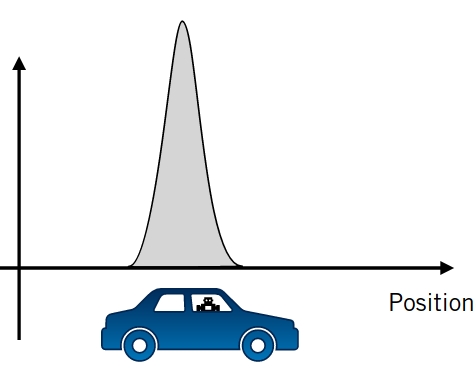
\includegraphics[width=0.8\textwidth]{./images/kalman_car.png}
%                 \caption{Exemplo Deslocamento Carro}
%             \end{figure}
        
%         Tempo contínuo
%         \begin{equation*}
%            \left\{
%             \begin{matrix}
%                 s = & s_0 + vt \\
%                 v = & v_0 + at
%             \end{matrix}, 
%             \quad
%             \mathbf{x} = 
%             \begin{bmatrix}
%                 x \\
%                 \dot{x}
%             \end{bmatrix},
%             \right.
%         \end{equation*}
        
%         \begin{equation*}
%             \text{e, }\mathbf{u}=a
%         \end{equation*}

%         \end{column}
%         \begin{column}[c]{0.6\textwidth}
            
%             \textbf{Eq. Movimento - Tempo Discreto}:

%             \begin{equation*}
%                 \mathbf{x}_t = 
%                 \begin{bmatrix}
%                         1 & \Delta t \\
%                         0 & 1
%                 \end{bmatrix}
%                 \mathbf{x}_{t-1} +
%                 \begin{bmatrix}
%                         0 \\
%                         \Delta t
%                 \end{bmatrix}
%                 \mathbf{u}_{t-1} +
%                 \mathbf{w}_{t-1}
%             \end{equation*}

%             \textbf{Eq. Sensor - Tempo Discreto}:

%             \begin{equation*}
%                 \mathbf{z}_t = 
%                 \begin{bmatrix}
%                         1 & 0
%                 \end{bmatrix}
%                 \mathbf{x}_{t} +
%                 v_{t}
%             \end{equation*}            

%             \textbf{Ruído}:

%             $\mathbf{w}_t \sim \mathcal{N} 
%                 \left(
%                     \begin{bmatrix}
%                     0 \\ 0    
%                     \end{bmatrix},
%                     \begin{bmatrix}
%                     0.1 & 0 \\
%                     0   & 0.1
%                 \end{bmatrix}
%                 \right)$ e :
            
%             $ v_t \sim \mathcal{N} (0,0.05)$

%         \end{column}
%     \end{columns}
% \end{frame}



% \begin{frame}[c]{Kalman Filter}
%     \framesubtitle{Exercício - Deslocamento Carro - Kalman Filter}
    
%     \begin{itemize}
%         \item 1) Dado o sistema que descreve o deslocamento do carro acima,
%         calcule o primeiro passo do algoritmo Kalman Filter.
%     \end{itemize}

%     \begin{columns}
%         \begin{column}[c]{0.4\textwidth}
%             \begin{figure}
%                 \centering
%                 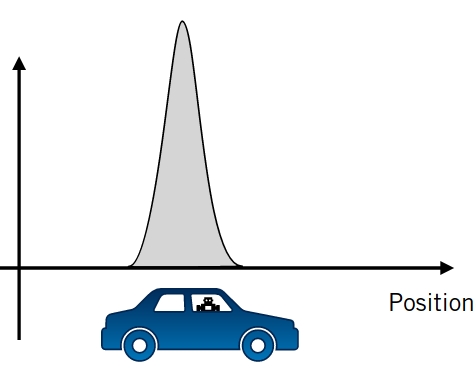
\includegraphics[width=0.8\textwidth]{./images/kalman_car.png}
%                 \caption{Exemplo Deslocamento Carro}
%             \end{figure}
            
%         \end{column}
%         \begin{column}[c]{0.6\textwidth}
            
%             \textbf{Condições Iniciais}:

%             \begin{equation*}
%                 \mu_0 \sim \mathcal{N} \left( 
%                     \begin{bmatrix}
%                         0 \\ 5
%                     \end{bmatrix}, 
%                     \begin{bmatrix}
%                         0.01 & 0 \\
%                         0 & 1
%                     \end{bmatrix} \right)
%             \end{equation*}

%             $\Delta t = 0.5s$

%             $u_0 = -2m/s^2$

%            $z_1 = 2.2 m$ 

%         \end{column}
%     \end{columns}
% \end{frame}


Extended Kalman Filter
\begin{itemize}
    \item \textcolor{red}{Sistema do Mundo Real não são lineares};
    \item O filtro de Kalman foi desenvolvido para sistemas lineares, e normalmente assume-se que todas as perturbações e ruídos podem ser descritos com uma distribuição gaussiana de média zero;
    \item \textcolor{blue}{Se qualquer uma das transições de estado ou equações de saída do sistema for uma função não linear}, o filtro de Kalman convencional pode não mais produzir uma estimativa de estado ideal. Para contornar o problema das não linearidades, um \textcolor{blue}{Extended Kalman Filter (EKF) foi desenvolvido}, onde as não linearidades do sistema são aproximadas com modelos lineares locais;
    \item \textbf{Portanto, o algoritmo EKF é comumente usado na prática};
\end{itemize}



\begin{itemize}
    \item Um exemplo clássico de sistemas considerado puramente linear é o do resistor,


\begin{figure}
    \centering
    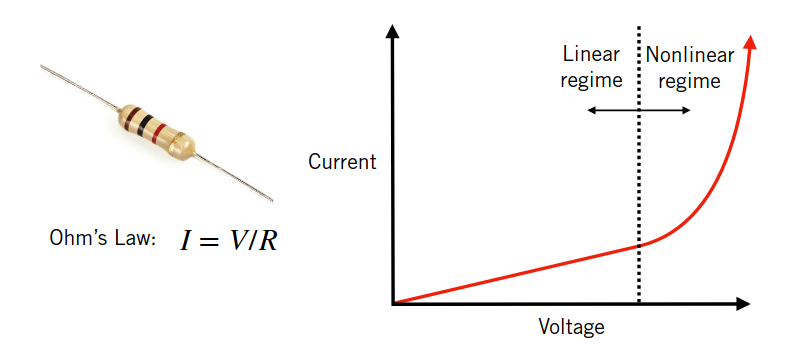
\includegraphics[width=0.8\textwidth]{chapters/chapter3/figures/resistor_curve.png}
    \caption{Curva experimental de corrente vs tensão Resistor}
\end{figure}

    \item Neste caso, o resistor tem um compartamento linear até determinada faixa de operação.
\end{itemize}



\begin{itemize}
    \item Problemas de Robótica Móvel mais realistas envolvem equação não lineares.
    \item Um sistema não linear pode ser escrito de uma forma geral:
    
    \begin{equation}
        \begin{split}
        x_t = & g(u_t, x_{t-1})\\
        z_t = & h(x_t)
        \end{split}
    \end{equation}
    
onde $g(u_t, x_{t-1})$ e $h(x_t)$ são funções não lineares que representam, consecutivamente, 
o modelo do sistema e o modelo dos sensores.

\end{itemize}


Linearização do Sistema



\begin{itemize}
    \item Podemos achar função linear do sistema no ponto $\color{red}{a}$ através da Expansão da Série de Taylor. Um exemplo interativo: 

\begin{figure}
    \centering
    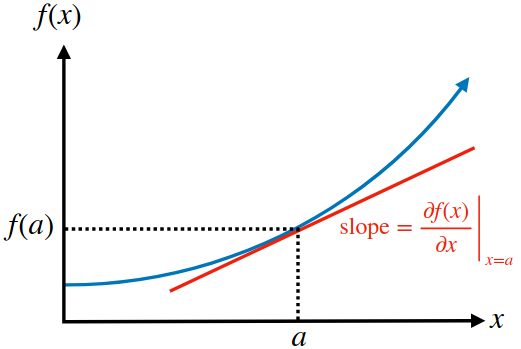
\includegraphics[width=0.4\textwidth]{chapters/chapter3/figures/taylor.png}
\end{figure}

\begin{equation}
    f(x) = \color{red}{f(a) + \left. \frac{\partial f(x)}{\partial x} \right\vert_{x=a}(x-a)} + 
    \color{gray}{\frac{1}{2!}\left. \frac{\partial^2 f(x)}{\partial^2 x} \right\vert_{x=a}(x-a)^2 + \cdots}
\end{equation}

    \item Para o EKF, \textcolor{red}{apenas a aproximação de primeira ordem é utilizada}.
\end{itemize}


Prediction
\begin{equation*}
    \begin{split}
        g(u_t, x_{t-1} \approx & g(u_t, \mu_{t-1}) + \frac{\partial g(u_t, \mu_{t-1}) }{\partial x_{t-1}}(x_{t-1}-\mu_{t-1}) \\
        g(u_t, x_{t-1} \approx & g(u_t, \mu_{t-1}) + \color{red}{G_t}\color{gray}{(x_{t-1}-\mu_{t-1})}
    \end{split}
\end{equation*}
            
onde $\color{red}G_t$ é calculado pela Matriz Jacobiana.

Measurement Update
\begin{equation*}
    \begin{split}
        h(x_t) \approx & h(\overline{\mu}_t) + \frac{\partial h(\overline{\mu}_t) }{\partial x_{t}}(x_{t}-\overline{\mu}_{t}) \\
        h(x_t) \approx & h(\overline{\mu}_t) + \color{blue}{H_t}\color{gray}{(x_{t}-\overline{\mu}_{t})}
    \end{split}
\end{equation*}
onde $\color{blue}H_t$ é calculado pela Matriz Jacobiana.


Linearização de sistemas

A matrix Jacobiana é data por:
\begin{equation*}
    \mathbb{J}
    =
    \frac{d \mathbf{f}}{d \mathbf{x}}
    =
    \left[ \frac{\partial \mathbf{f}}{\partial q_1}
        \cdots \frac{\partial \mathbf{f}}{\partial x_n} \right]
    =
    \begin{bmatrix}
        \frac{\partial f_1}{\partial x_1} & \cdots &
        \frac{\partial f_1}{\partial x_n}                   \\
        \vdots                            & \ddots & \vdots \\
        \frac{\partial f_m}{\partial x_1} & \cdots &
        \frac{\partial f_m}{\partial x_n}
    \end{bmatrix}
\end{equation*}
    

dado um sistema representado por $\mathbf{F(x)}$, calcule a
    matriz jacobina do sistema:
    
    \begin{equation*}
        \mathbf{F(x)}
        =
        \begin{bmatrix}
            f_1 \\
            f_2
        \end{bmatrix}
        =
        \begin{bmatrix}
            x_1 + x_2 \\
            x_1^2
        \end{bmatrix}
    \end{equation*}
    
    logo:

    \begin{equation*}
        \frac{d \mathbf{f(x)}}{d \mathbf{x}}
        =
        \begin{bmatrix}
            \frac{\partial f_1}{\partial x_1} &
            \frac{\partial f_1}{\partial x_2} \\
            \frac{\partial f_2}{\partial x_1} &
            \frac{\partial f_2}{\partial x_2}
        \end{bmatrix}
        =
        \begin{bmatrix}
            1 & 1 \\
            2x_1 & 0
        \end{bmatrix}
    \end{equation*}

Algoritmo

\begin{algorithm}[H]
    \caption{Extended-Kalman-Filter}
    \begin{algorithmic}[1]
    \Procedure{Prediction}{$\mu_{t-1}, {\textstyle\sum}_{t-1}, u_t$}
        \State $\overline{\mu}_t = g(u_t, \mu_{t-1})$
        \State $ \overline{\textstyle\sum}_t = G_t {\textstyle\sum}_{t-1} G_t^T+ Q_t$ 
        \State \textbf{Return} $\left(\overline{\mu}_t, \overline{\textstyle\sum}_t\right)$
    \EndProcedure
    \Procedure{Update}{$\overline{\mu}_{t}, \overline{\textstyle\sum}_{t}, z_t$}
        \State $K_t = \overline{\textstyle\sum}_tH_t^T(H_t\overline{\textstyle\sum}_tH_t^T+R_t)^{-1}$
        \State $\mu_t  = \overline{\mu}_t + K_t(z_t -h(\overline\mu_t))$
        \State{$\textstyle\sum_t = (I-K_t H_t)\overline{\textstyle\sum}_t$}
        \State \textbf{Return} $\left(\mu_t, \textstyle\sum_t\right)$
    \EndProcedure
    \end{algorithmic}
\end{algorithm}


% \begin{frame}[c]{Extended Kalman Filter}
%     \framesubtitle{Exercício - Deslocamento Carro - Extended Kalman Filter}    \begin{columns}
%         \begin{column}[c]{0.4\textwidth}
%             \begin{figure}
%                 \centering
%                 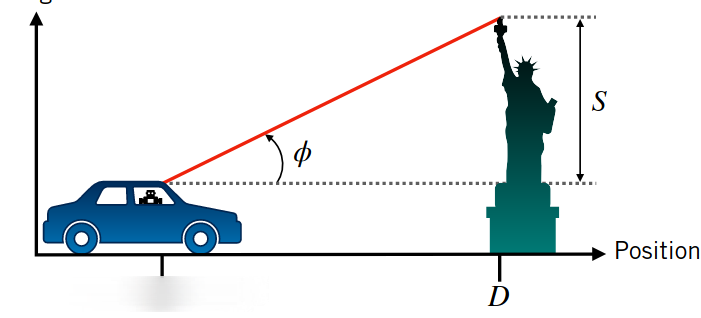
\includegraphics[width=1\textwidth]{./images/kalman_car2.png}
%                 \caption{Exemplo Deslocamento Carro}
%             \end{figure}
        
%         Tempo contínuo
%         \begin{equation*}
%            \left\{
%             \begin{matrix}
%                 s = & s_0 + vt \\
%                 v = & v_0 + at
%             \end{matrix}, 
%             \quad
%             \mathbf{x} = 
%             \begin{bmatrix}
%                 x \\
%                 \dot{x}
%             \end{bmatrix},
%             \right.
%         \end{equation*}
        
%         \begin{equation*}
%             \text{e, }\mathbf{u}=a
%         \end{equation*}

%         \end{column}
%         \begin{column}[c]{0.6\textwidth}
            
%             \textbf{Eq. Movimento - Tempo Discreto}:

%             \begin{equation*}
%                 \mathbf{x}_t = 
%                 \begin{bmatrix}
%                         1 & \Delta t \\
%                         0 & 1
%                 \end{bmatrix}
%                 \mathbf{x}_{t-1} +
%                 \begin{bmatrix}
%                         0 \\
%                         \Delta t
%                 \end{bmatrix}
%                 \mathbf{u}_{t-1} +
%                 \mathbf{w}_{t-1}
%             \end{equation*}

%             \textbf{Eq. Sensor - Tempo Discreto}:

%             \begin{equation*}
%                 \mathbf{z}_t = \phi_t  = 
%                 \tan^{-1}\left(\frac{S}{D-x_t} \right) +
%                 v_{t}
%             \end{equation*}            

%             \textbf{Ruído}:

%             $\mathbf{w}_t \sim \mathcal{N} 
%                 \left(
%                     \begin{bmatrix}
%                     0 \\ 0    
%                     \end{bmatrix},
%                     \begin{bmatrix}
%                     0.1 & 0 \\
%                     0   & 0.1
%                 \end{bmatrix}
%                 \right)$ e :
            
%             $ v_t \sim \mathcal{N} (0,0.05)$

%         \end{column}
%     \end{columns}
% \end{frame}



% \begin{frame}[c]{Extended Kalman Filter}
%     \framesubtitle{Exercício - Deslocamento Carro - Extended Kalman Filter}
    
%     \begin{itemize}
%         \item 1) Dado o sistema que descreve o deslocamento do carro acima,
%         calcule o primeiro passo do algoritmo Extended Kalman Filter.
%     \end{itemize}

%     \begin{columns}
%         \begin{column}[c]{0.4\textwidth}
%             \begin{figure}
%                 \centering
%                 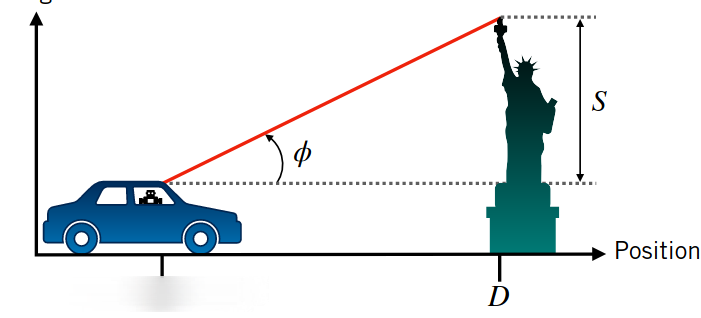
\includegraphics[width=1\textwidth]{./images/kalman_car2.png}
%                 \caption{Exemplo Deslocamento Carro}
%             \end{figure}
            
%         \end{column}
%         \begin{column}[c]{0.6\textwidth}
            
%             \textbf{Condições Iniciais}:

%             \begin{equation*}
%                 \mu_0 \sim \mathcal{N} \left( 
%                     \begin{bmatrix}
%                         0 \\ 5
%                     \end{bmatrix}, 
%                     \begin{bmatrix}
%                         0.01 & 0 \\
%                         0 & 1
%                     \end{bmatrix} \right)
%             \end{equation*}

%             $\Delta t = 0.5s$

%             $u_0 = -2m/s^2$

%            $z_1 = \frac{\pi}{6} rad$ 

%            $D = 40m$

%            $S = 20m$

%         \end{column}
%     \end{columns}
% \end{frame}




% \section{Glossary}
% \begin{Glossary}
% \item[360 Degree Review] Performance review that includes feedback from superiors, peers, subordinates, and clients.
% \item[Abnormal Variation] Changes in process performance that cannot be accounted for by typical day-to-day variation. Also referred to as
% non-random variation.
% \item[Acceptable Quality Level (AQL)] The minimum number of parts that must comply with quality standards, usually stated as a percentage.
% \item[Activity] The tasks performed to change inputs into outputs.
% \item[Adaptable] An adaptable process is designed to maintain effectiveness and efficiency as requirements change. The process is
% deemed adaptable when there is agreement among suppliers, owners, and customers that the process will meet
% requirements throughout the strategic period.
% \end{Glossary}



